\documentclass[12pt]{article}

\title{Activity 10: Classes}
\author{Dr. Chris Mayfield}
\date{CS 149, Fall 2016}

%\ProvidesPackage{cspogil}

% fonts
\usepackage[utf8]{inputenc}
\usepackage[T1]{fontenc}
\usepackage{mathpazo}

% spacing
\usepackage[margin=2cm]{geometry}
\renewcommand{\arraystretch}{1.4}
\setlength{\parindent}{0pt}

% orphans and widows
\clubpenalty=10000
\widowpenalty=10000
\pagestyle{empty}

% figures and tables
\usepackage{graphicx}
\usepackage{multicol}
\usepackage{tabularx}
\usepackage{wrapfig}

% fixed-width columns
\usepackage{array}
\newcolumntype{L}[1]{>{\raggedright\let\newline\\\arraybackslash\hspace{0pt}}m{#1}}
\newcolumntype{C}[1]{>{\centering\let\newline\\\arraybackslash\hspace{0pt}}m{#1}}
\newcolumntype{R}[1]{>{\raggedleft\let\newline\\\arraybackslash\hspace{0pt}}m{#1}}

% include paths
\makeatletter
\def\input@path{{Models/}{../../Models/}}
\graphicspath{{Models/}{../../Models/}}
\makeatother

% colors
\usepackage[svgnames,table]{xcolor}
\definecolor{bgcolor}{HTML}{FAFAFA}
\definecolor{comment}{HTML}{007C00}
\definecolor{keyword}{HTML}{0000FF}
\definecolor{strings}{HTML}{B20000}

% table headers
\newcommand{\tr}{\bf\cellcolor{Yellow!10}}

% syntax highlighting
\usepackage{textcomp}
\usepackage{listings}
\lstset{
    basicstyle=\ttfamily\color{black},
    backgroundcolor=\color{bgcolor},
    numberstyle=\scriptsize\color{comment},
    commentstyle=\color{comment},
    keywordstyle=\color{keyword},
    stringstyle=\color{strings},
    columns=fullflexible,
    keepspaces=true,
    showlines=true,
    showstringspaces=false,
    upquote=true
}

% code environments
\newcommand{\java}[1]{\lstinline[language=java]{#1}}%[
\lstnewenvironment{javalst}{\lstset{language=java,backgroundcolor=}}{}
\lstnewenvironment{javabox}{\lstset{language=java,frame=single,numbers=left}\quote}{\endquote}

% PDF properties
\usepackage[pdftex]{hyperref}
\urlstyle{same}
\makeatletter
\hypersetup{
  pdftitle={\@title},
  pdfauthor={\@author},
  pdfsubject={\@date},
  pdfkeywords={},
  bookmarksopen=false,
  colorlinks=true,
  citecolor=black,
  filecolor=black,
  linkcolor=black,
  urlcolor=blue
}
\makeatother

% titles
\makeatletter
\renewcommand{\maketitle}{\begin{center}\LARGE\@title\end{center}}
\makeatother

% boxes [optional height]
\newcommand{\emptybox}[1][10em]{
\vspace{1em}
\begin{tabularx}{\linewidth}{|X|}
\hline\\[#1]\hline
\end{tabularx}}

% models
\newcommand{\model}[1]{\section{#1}\nopagebreak}
\renewcommand{\thesection}{Model~\arabic{section}}

% questions
\newcommand{\quest}[1]{\subsection*{Questions~ (#1)}}
\newcounter{question}
\newcommand{\Q}{\vspace{1em}\refstepcounter{question}\arabic{question}.~ }
\renewcommand{\thequestion}{\#\arabic{question}}

% sub-question lists
\usepackage{enumitem}
\setenumerate[1]{label=\alph*)}
\setlist{itemsep=1em,after=\vspace{1ex}}

% inline answers
\definecolor{answers}{HTML}{C0C0C0}
\newcommand{\ans}[1]{%
\ifdefined\Student
    \leavevmode\phantom{~~\textcolor{answers}{#1}}
\else
    ~~\textcolor{answers}{#1}
\fi}

% longer answers [optional height]
\newsavebox{\ansbox}
\newenvironment{answer}[1][4em]{
\nopagebreak
\begin{lrbox}{\ansbox}
\begin{minipage}[t][#1]{\linewidth}
\color{answers}
}{
\end{minipage}
\end{lrbox}
\ifdefined\Student
    \phantom{\usebox{\ansbox}}%
\else
    \usebox{\ansbox}%
\fi}


\begin{document}

\maketitle

When you define a class in Java, you are defining a new data type.
Classes have \emph{attributes} (data) and \emph{methods} (code).
A \emph{class diagram} is a graphical summary of the attributes and methods.

\model{Die objects}
\label{CS1/class-die}

\begin{quote}
\hfill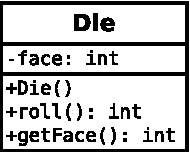
\includegraphics{CS1/Die.pdf}
\vspace*{-84pt}

\begin{javalst}
/**
 * Simulates a Die object.
 */
public class Die {
    
    private int face;
    
    /**
     * Constructs a new die with a random face value.
     */
    public Die() {
        face = 1;
    }
    
    /**
     * Gets the current face value of the die.
     *
     * @return current face value of the die
     */
    public int getFace() {
        return face;
    }
    
    /**
     * Simulates the roll of the die.
     *
     * @return new face value of the die
     */
    public int roll() {
        face = (int) (Math.random() * 6) + 1;
        return face;
    }
    
}
\end{javalst}

\vspace*{-128pt}
% https://commons.wikimedia.org/wiki/File:2-Dice-Icon.svg
\hfill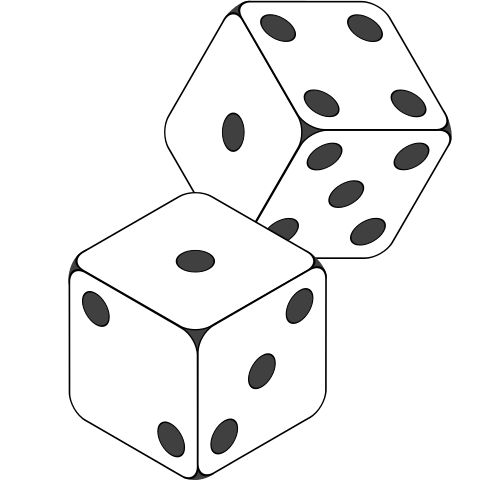
\includegraphics[width=2in]{CS1/dice.png}
\end{quote}


\quest{10 min}


\Q What are the attributes of \java{Die}? What are the methods?

\begin{answer}
The only attribute is \java{face}. The methods are \java{Die}, \java{roll}, and \java{getFace}.
\end{answer}


\Q In the class diagram, what do the \java{-} and \java{+} symbols represent? What does the \java{:} represent?

\begin{answer}
Plus means {\tt public}, minus means {\tt private}, and colon refers to the data type.
\end{answer}


\Q Write a statement that \emph{declares} a \java{Die} variable named \java{lucky}.

\begin{answer}
\tt Die lucky;
\end{answer}


\Q Each \emph{instance} of a class (in memory) is called an object. Write a statement that \emph{instantiates} a \java{new} \java{Die} object and assigns it to \java{lucky}.

\begin{answer}
\tt lucky = new Die();
\end{answer}


\Q When you instantiate an object, you invoke a \emph{constructor}.
This method has no return type and has the same name as the class itself. What does the \java{Die} constructor do?

\begin{answer}
It ``rolls'' the die by calling the \java{roll} method.
\end{answer}


\Q Notice how the \java{roll} method refers to \java{face}, yet that variable is not declared in the method. What does the \java{roll} method change, in terms of the \java{Die} object?

\begin{answer}
It updates the value of the \java{face} attribute.
\end{answer}


\Q What is the purpose of the \java{getFace} method? Show how you would use it in a \java{main} method of another class.

\begin{answer}
It updates the value of the \java{face} attribute. In a {\tt main} method, you would do something like: {\tt System.out.println(lucky.getFace());}
\end{answer}

\model{Circle objects}
\label{CS1/class-circle}

Unified Modeling Language (UML) provides a way of graphically illustrating a class’s design, independent of the programming language.

\begin{center}
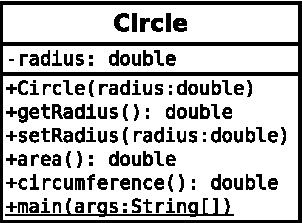
\includegraphics{CS1/Circle.pdf}
\end{center}


\quest{15 min}


\Q What are the attributes and methods of \java{Circle}, and what is their \emph{visibility}?

\begin{answer}
The attribute \java{radius} is private, and the methods \java{Circle}, \java{area}, \java{circumference}, \java{getRadius}, and \java{setRadius} are public.
\end{answer}


\Q Based on \ref{CS1/class-die} and \ref{CS1/class-circle}, what is typically \java{public} and what is typically \java{private}?

\begin{answer}
Attributes are typically private, and methods are typically public.
\end{answer}


\Q How would you declare a variable named \java{unit} that is a \java{Circle} object?
How would you instantiate a circle with a radius of 1.0 and assign it to \java{unit}?

\begin{answer}
\tt Circle unit;

\tt unit = new Circle(1.0);
\end{answer}


\Q Write the code (inside {\tt Circle.java}) that declares the \java{radius} attribute.

\begin{answer}
\tt private double radius;
\end{answer}


\Q Write the code for \java{getRadius}. (Don't worry about Javadoc comments for this activity.)

\begin{answer}[5em]
\begin{javaans}
    public double getRadius() {
        return radius;
    }
\end{javaans}
\end{answer}


\Q Write the code for \java{setRadius}. Note there are two variables named \java{radius}: the parameter of \java{setRadius}, and \java{this.radius} for the object itself. Before you set the radius, first check if the parameter is negative, and if it is, set the radius to zero instead.

\begin{answer}[11em]
\begin{javaans}
    public void setRadius(double radius) {
        if (radius >= 0) {
            this.radius = radius;
        }
        else {
            this.radius = 0;
        }
    }
\end{javaans}
\end{answer}


\Q Write the complete code for \java{area} and \java{circumference}.
The area of a circle is $\pi r^2$, and the circumference is $2 \pi r$.
Ideally, each method should be one line of code.

\begin{answer}[10em]
\begin{javaans}
    public double area() {
        return Math.PI * radius * radius;
    }

    public double circumference() {
        return 2.0 * Math.PI * radius;
    }
\end{javaans}
\end{answer}


\Q Write a \java{main} method that creates a \java{Circle} object with a radius of 2.0 and displays its area and circumference on the screen.

\begin{answer}[7em]
\begin{javaans}
    public static void main(String[] args) {
        Circle big = new Circle(2.0);
        System.out.println("big area = " + big.area());
        System.out.println("big circ = " + big.circumference());
    }
\end{javaans}
\end{answer}

\newpage
\model{Case Study: Let's Make a Deal}

It was mid-semester and the pressure was on, not only in CS but in other classes.
Jamie and Pat were each working on the programming assignment in the lab, but neither was having much success.
Jamie had started several days ago, but he was having trouble debugging his current work.
Pat had just started that day and knew that she would be turning it in late.
Regardless, Pat offered to help Jamie work out the problems with his code.

\vspace{1em}

Together, and after a couple of hours of work, they got the program to work.
Pat said, ``Now that yours is working, can you give me the code so that I can also get credit for this assignment?''
When Jamie objected, Pat said, ``Hey, you wouldn't have gotten it finished if it weren't for my help, and now mine will be even later!''
So Jamie turned over a copy of the code.
Pat made some changes to a few sections, and then turned in the final program.


\quest{10 min}


\Q Which, if any, of the students were at fault? Why?

\begin{answer}[6em]
\end{answer}


\Q Which specific Honor Code violations occurred?

\begin{answer}[6em]
\end{answer}


\Q What should Pat have done in this situation?

\begin{answer}[6em]
\end{answer}


\Q What should Jamie have done in this situation?

\begin{answer}[6em]
\end{answer}

\newpage
\section*{Case Study: A Friendly Assist}

George was struggling with the programming assignment on the night it was due.
He had gone home over the weekend before, thinking that it would be easy to do this assignment, but it turned out to be more difficult than he thought.
After working on some parts of it and giving up in frustration, he turned to Shelley, a senior CS student who had taken the course several semesters before.
He showed Shelley the assignment, and the two of them worked on it late into the night.
They successfully submitted the program with a late penalty of only one day.


\quest{10 min}


\Q Which, if any, of the students were at fault? Why?

\begin{answer}[6em]
\end{answer}


\Q Which specific Honor Code violations occurred?

\begin{answer}[6em]
\end{answer}


\Q What should Shelley have done in this situation?

\begin{answer}[6em]
\end{answer}


\Q What options did George have besides cheating?

\begin{answer}[6em]
\end{answer}


\end{document}
